\section{Event storage}
\textbf{Apache Kafka}
\textbf{Durable storage - criterion 1.1}

In Kafka, records are stored in partitions each of which is stored on the disk as a number of segment files \cite{kafkadocumentation}. The broker receives records and writes them sequentially to these files. When a segment file reaches its configurable maximum size, a new file will be created for writing new records. Since all records are only appended to these files, the read/write of records only requires sequential I/O on the disk. This is one of the key design features of Kafka to help maintain fast performance even on cheap hard disks.  

However, a Kafka broker can already acknowledge writing requests when records are written to I/O buffer and not necessarily when records are persisted to disk. Therefore, durability is not guaranteed, and message loss can still happen when the broker fails before flushing records to disk. User can force disk flush to ensure durability whenever a message is received but this is not recommended by Kafka since it can reduce the throughput of the system \cite{kafkadocumentation}. To achieve durability, a more common approach is combining this unflushed write feature with redundant write on other brokers in the cluster which is the fault-tolerance feature for storage provided by Kafka. This is elaborated in more detail in the next section.

\textbf{Event storage is fault tolerant - criterion 10.1}\\
As briefly mentioned in the general concept, there are two types of Kafka partitions, namely, leader and follower. The leader partition is active and can serve read/write requests from clients while followers are standby replicas of the leader. For fault tolerance, Kafka supports data replication among brokers in the cluster \cite{kafkadatareplication}. For each topic, user can specify a replication factor which determines the number of existing copies of records on Kafka.  When replication factor is 2 or more, every partition of the topic will have 1 leader and 1 or more followers. For each partition, each of its copies will be distributed on a different broker in the cluster. Therefore, there will be no single point of failure for record storage. The replication factor must be equal or smaller than the number of brokers in the Kafka cluster.

However, enabling only data replication on the broker cannot guarantee that all records are safely replicated on the Kafka cluster.  By default, a Kafka producer sends a record and only waits for the acknowledgement of successful write from the leader partition. If the broker with the leader partition goes down before the record is flushed to its disk and replicated to other follower replications, the record may be lost without the producer knowing about it for resending. Therefore, the producer must be strictly configured to wait for acknowledgements from the leader partition as well as other follower replicas. In this case, the leader partition will also wait for acknowledgements from its followers before confirming with client. By having the redundant acknowledgements, durability is guaranteed even when messages are not yet persisted to disks given that all brokers retain the partition do not fail simultaneously. 
\begin{figure}[h]
	\centering
	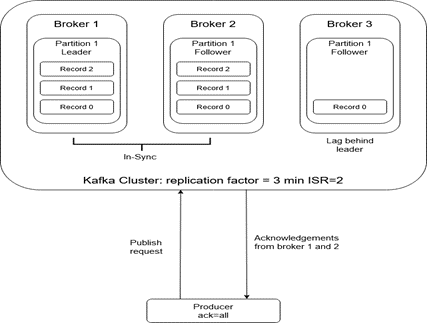
\includegraphics[width=8cm,height=6.5cm]{images/ft-eventstorage-kafka.png}
	\caption{Data replication model for fault tolerance of event storage on Kafka.}
	\label{fig:fteventstorekafka}
\end{figure}

For each replicated partition, the follower periodically fetch data from leader to stay in-sync. If the producer waits for acknowledgements from all replicas, some followers may fall too far behind the leader for instance due to network connection and increase the waiting time of the producer. Therefore, the leader of the partition dynamically maintains a list of in-sync replicas (ISR) which contains itself and all followers which currently stays synchronized with it. This list is stored on Zookeeper. When a follower does not catch up with the leader by sending fetch request after a configured amount of time, it will be removed from the ISR of the partition. The slow follower can rejoin ISR later when it has fully caught up with the leader partition. In practice, the producer will only wait for acknowledgements from the ISR instead of all replicas. This aims at balancing between the durability, fault-tolerance of published records and the latency for acknowledgment. As a result, a message acknowledged to producer can survive up to ISR-1 failed nodes and still be available to consumer.

It could be possible that all followers of a partition are out-of-sync with the leader. In this case, producer only receives one acknowledgment from the leader which brings back the problem of losing messages. Therefore, Kafka also provides the option to configure the minimum number of in-sync replicas. If the ISR falls below this number, new writing requests will be rejected, and availability is compromised to ensure the durability.

Durability and fault tolerance of data storage on Kafka are closely related to each other and can only be achieved with the right configurations on both Kafka brokers and Kafka producers. In addition, Kafka provides many configuration options to give users the flexibility to choose different priorities for their systems such as availability, durability, latency. 

\textbf{Flexible data retention policy - criterion 1.2}\\
All records published to Kafka will be retained. Old data can be cleaned up with different cleanup policies \cite{kafkadocumentation}. These policies can be configured on the broker level which will then be applied to all topics or they can be configured differently for individual topic. There are two basic strategies to retain data:
\begin{itemize}
	\item Delete: All records are retained for a period of time or based on a maximum size and then they will be deleted.
	\item Compact: This strategy is only applicable to records with key values. The topic will be compacted. Only the latest record of each key value is retained.
\end{itemize}

For the first strategy, user can choose different retention policies for a partition based on maximum size or for a segment file of a partition based on retention period. Once the retention limit is exceeded, oldest segment file of the partition will be deleted. By default, there is no limit on the size of a partition and the retention period is 7 days. User can also configure infinite retention period if necessary.

\begin{figure}[h]
	\centering
	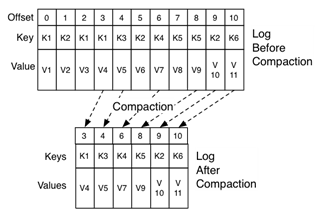
\includegraphics[width=6.5cm,height=5.5cm]{images/compact-kafka.png}
	\caption{Log compaction on Kafka (taken from Kafka documentation \cite{kafkadocumentation}).}
	\label{fig:compactekafka}
\end{figure}
For the second strategy, the background cleaner thread of Kafka will regularly scan the segment files and keep only the latest record for each key value (Figure \ref{fig:compactekafka}). Therefore, this only works with records with non-empty key value. Writing request of record without a key to a topic configured with compact cleanup policy will be rejected.


The two strategies can also be combined. With this setup, topics will be compacted regularly but when the retention maximum size or maximum retention period is reached, the data will also be removed regardless of being compacted or not. For example, in case of an online shopping application where each order is kept track by a sequence of events published to Kafka as records, when users are interested in the latest status of an order but only if the order is not older than 3 months, it is reasonable to this combination of retention strategies.

To sum up, Kafka provides a flexible way to retain all records or only selective data. Users can choose the appropriate strategy based on their use cases. 





